The expected number of signal and background events for an integrated 
luminosity of 1\ifb{} after applying the $\WW$ like selection are reported in 
Tables~\ref{tab:wwselection0}(0-jet),~\ref{tab:wwselection1}(1-jet), 
and~\ref{tab:wwselection2}(2-jet). The selection includes that none of the 
jets are top-tagged. In addition, the angle between the dilepton 
system and the jet in the transverse plane must be smaller than 165 dg. in 
the $ee/\mu\mu$ final states for the 1-jet bin. The $gg \to H \to WW$ 
simulated events are reweighted to match the Higgs $\pt$ at NNLO, as explained 
in Section~\ref{sec:datasets}; all data-driven corrections are not applied. The 
corresponding $\Delta\phi$, di-lepton mass, di-lepton $p_T$, $M_T$ and projected 
$\met$ distributions are shown in Figs.~\ref{fig:dPhi_jets0}-\ref{fig:pmet_jets0}(0-jet) 
and Figs.~\ref{fig:dPhi_jets1}-\ref{fig:pmet_jets1}(1-jet).

\begin{table}[!ht]
  \begin{center}
 {\scriptsize
  \begin{tabular} {|c|c|c|c|c|c|c|c|c|c|c|}
\hline
 & $\dy$ & $\ttbar$ & single-top & $\Wjets$ & $\WZ+\ZZ$ & $gg \to WW$ & $qq \to WW$ & H$_{130}$ &   H$_{160}$ \\
  \hline
  \hline
  $\M\M$   &  2.5 $\pm$   1.5 &  6.1 $\pm$   0.9 &  2.7 $\pm$	0.2 &	6.2 $\pm$   3.6&  4.8 $\pm$   0.2 &  4.3 $\pm$   0.1 & 76.1 $\pm$   0.7 &  9.9 $\pm$   0.1 & 31.0 $\pm$   0.4\\
  $\E\M$   &  2.5 $\pm$   1.5 &  8.3 $\pm$   1.1 &  3.9 $\pm$   0.3 &  20.8 $\pm$   6.6&  2.7 $\pm$   0.1 &  5.2 $\pm$   0.1 &106.3 $\pm$   0.8 & 10.0 $\pm$   0.1 & 29.0 $\pm$   0.3\\
  $\M\E$   &  0.0 $\pm$   0.0 &  8.7 $\pm$   1.1 &  4.1 $\pm$   0.3 &  27.0 $\pm$   7.5&  3.7 $\pm$   0.2 &  5.6 $\pm$   0.1 &118.6 $\pm$   0.9 & 12.2 $\pm$   0.2 & 30.6 $\pm$   0.3\\
  $\E\E$   &  3.5 $\pm$   1.7 &  3.1 $\pm$   0.7 &  2.3 $\pm$   0.2 &  14.6 $\pm$   5.5&  2.9 $\pm$   0.1 &  3.0 $\pm$   0.1 & 48.4 $\pm$   0.5 &  5.7 $\pm$   0.1 & 19.7 $\pm$	  0.3\\
  \hline
       all &  8.5 $\pm$   2.7 & 26.3 $\pm$   1.9 & 13.1 $\pm$   0.5 &  68.6 $\pm$  11.9& 14.1 $\pm$   0.3 & 18.1 $\pm$   0.2 &349.3 $\pm$   1.5 & 37.9 $\pm$   0.3 &110.2 $\pm$   0.7\\
 \hline
  \end{tabular}
  }
  \caption{Expected number of signal and background events for an 
  integrated luminosity of 1\ifb{} after applying the \ww\ 
  0-jet selection requirements. Monte Carlo statistical 
  uncertainties are included.}
   \label{tab:wwselection0}
  \end{center}
\end{table}

\begin{table}[!ht]
  \begin{center}
 {\scriptsize
  \begin{tabular} {|c|c|c|c|c|c|c|c|c|c|c|}
\hline
  & $\dy$ & $\ttbar$ & single-top & $\Wjets$ & $\WZ+\ZZ$ & $gg \to WW$ & $qq \to WW$ & H$_{130}$ &   H$_{160}$ \\
  \hline
  \hline
  $\M\M$   &  7.6 $\pm$   2.5 & 14.3 $\pm$   1.4 &  4.7 $\pm$	0.3 &	2.1 $\pm$	2.1 &  1.6 $\pm$	0.1 &  1.2 $\pm$	0.0 & 21.0 $\pm$	0.4 &  3.0 $\pm$	0.1 & 11.5 $\pm$	0.2 \\
  $\E\M$   &  3.5 $\pm$   1.7 & 22.6 $\pm$   1.8 &  6.5 $\pm$	0.4 &	4.2 $\pm$	2.9 &  2.2 $\pm$	0.1 &  1.6 $\pm$	0.0 & 31.0 $\pm$	0.4 &  3.9 $\pm$	0.1 & 12.5 $\pm$	0.2 \\
  $\M\E$   &  6.4 $\pm$   2.4 & 26.9 $\pm$   1.9 &  7.9 $\pm$	0.4 &	4.2 $\pm$	2.9 &  3.4 $\pm$	0.2 &  2.0 $\pm$	0.1 & 34.5 $\pm$	0.5 &  4.5 $\pm$	0.1 & 13.4 $\pm$	0.2 \\
  $\E\E$   &  4.2 $\pm$   1.9 & 11.5 $\pm$   1.2 &  3.3 $\pm$	0.3 &	4.2 $\pm$	2.9 &  1.9 $\pm$	0.1 &  0.8 $\pm$	0.0 & 13.4 $\pm$	0.3 &  1.9 $\pm$	0.1 &  7.5 $\pm$	0.1 \\
  \hline
       all & 21.6 $\pm$   4.3 & 75.3 $\pm$   3.2 & 22.4 $\pm$   0.7 &  14.6 $\pm$	5.5 &  9.2 $\pm$	0.3 &  5.7 $\pm$	 0.1 & 99.8 $\pm$	 0.8 & 13.4 $\pm$	 0.1 & 44.9 $\pm$	 0.3 \\
 \hline
  \end{tabular}
  }
  \caption{Expected number of signal and background events for an 
  integrated luminosity of 1\ifb{} after applying the \ww\ 
  1-jet selection requirements. Monte Carlo statistical 
  uncertainties are included.}
   \label{tab:wwselection1}
  \end{center}
\end{table}

\begin{table}[!ht]
  \begin{center}
 {\scriptsize
  \begin{tabular} {|c|c|c|c|c|c|c|c|c|c|c|}
\hline
  & $\dy$ & $\ttbar$ & single-top & $\Wjets$ & $\WZ+\ZZ$ & $gg \to WW$ & $qq \to WW$ & H$_{130}$ &   H$_{160}$ \\
  \hline
  \hline
  $\M\M$   & 12.7 $\pm$   3.5 & 18.8 $\pm$   1.6 &  1.6 $\pm$	0.2 &	0.0 $\pm$ 0.0 &  0.6 $\pm$   0.1 &  0.2 $\pm$	0.0 &  4.7 $\pm$   0.2 &  1.2 $\pm$   0.0 &  4.3 $\pm$   0.1 \\
  $\E\M$   &  1.9 $\pm$   1.4 & 25.6 $\pm$   1.9 &  2.3 $\pm$	0.2 &	0.0 $\pm$ 0.0 &  0.5 $\pm$   0.1 &  0.3 $\pm$	0.0 &  6.1 $\pm$   0.2 &  1.3 $\pm$   0.0 &  4.0 $\pm$   0.1 \\
  $\M\E$   &  3.7 $\pm$   1.9 & 30.0 $\pm$   2.0 &  3.4 $\pm$	0.3 &	0.0 $\pm$ 0.0 &  0.8 $\pm$   0.1 &  0.3 $\pm$	0.0 &  7.4 $\pm$   0.2 &  1.5 $\pm$   0.0 &  4.6 $\pm$   0.1 \\
  $\E\E$   &  8.4 $\pm$   2.7 & 12.8 $\pm$   1.3 &  1.3 $\pm$	0.2 &	2.1 $\pm$ 2.1 &  0.5 $\pm$   0.1 &  0.1 $\pm$	0.0 &  3.2 $\pm$   0.1 &  0.6 $\pm$   0.0 &  2.6 $\pm$   0.1 \\
  \hline
       all & 26.7 $\pm$   5.0 & 87.3 $\pm$   3.5 &  8.6 $\pm$   0.4 &   2.1 $\pm$ 2.1 &  2.5 $\pm$   0.2 &  1.0 $\pm$   0.0 & 21.4 $\pm$   0.4 &  4.6 $\pm$   0.1 & 15.4 $\pm$   0.2 \\
 \hline
  \end{tabular}
  }
  \caption{Expected number of signal and background events for an 
  integrated luminosity of 1\ifb{} after applying the \ww\ 
  2-jet selection requirements. Monte Carlo statistical 
  uncertainties are included.}
   \label{tab:wwselection2}
  \end{center}
\end{table}


\begin{figure}[!hbtp]
\centering
\subfigure[]{
\centering
\label{subfig:dPhi_hm120_jets0}
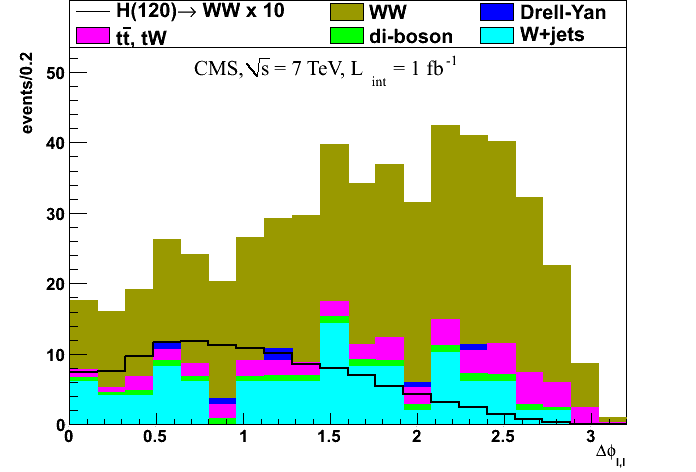
\includegraphics[width=.32\textwidth]{figures/dPhi_hm120_jets0.png}}
\subfigure[]{
\centering
\label{subfig:dPhi_hm160_jets0}
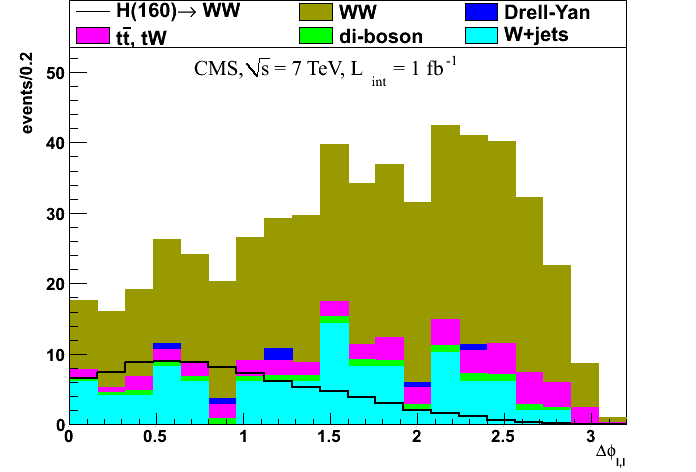
\includegraphics[width=.32\textwidth]{figures/dPhi_hm160_jets0.png}}
\subfigure[]{
\centering
\label{subfig:dPhi_hm250_jets0}
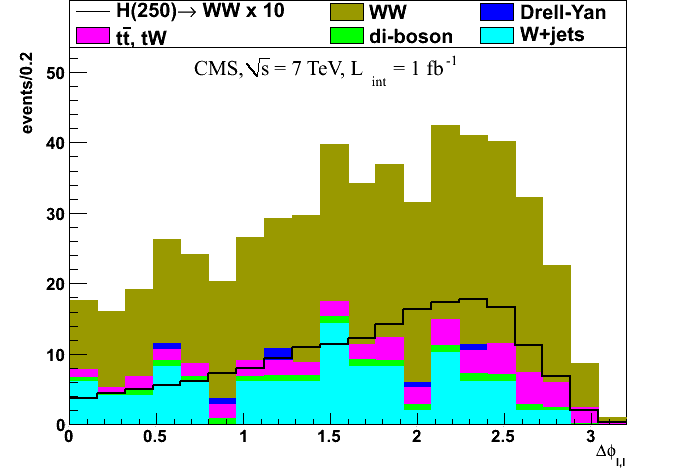
\includegraphics[width=.32\textwidth]{figures/dPhi_hm250_jets0.png}}\\
\caption{Lepton $\Delta\phi$ distribution after \WW\ selection for $m_H$=120 $\GeVcc$ \subref{subfig:dPhi_hm120_jets0}, 
$m_H$=160 $\GeVcc$ \subref{subfig:dPhi_hm160_jets0} and $m_H$=250 $\GeVcc$ \subref{subfig:dPhi_hm250_jets0} in the 0-jet bin.}
\label{fig:dPhi_jets0}
\end{figure}

\begin{figure}[!hbtp]
\centering
\subfigure[]{
\centering
\label{subfig:dilepmass_hm120_jets0}
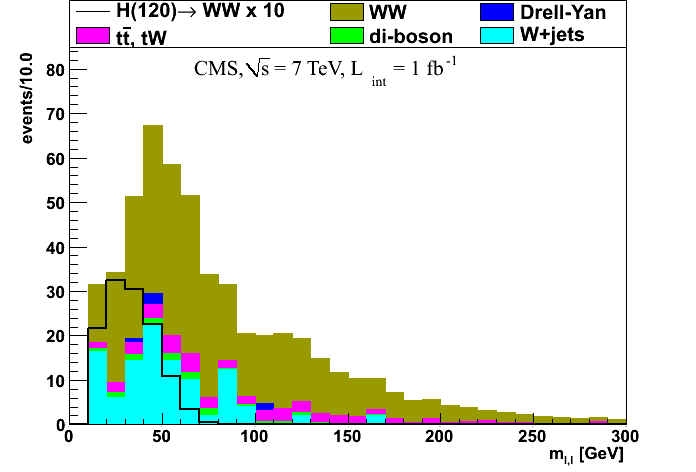
\includegraphics[width=.32\textwidth]{figures/dilepmass_hm120_jets0.png}}
\subfigure[]{
\centering
\label{subfig:dilepmass_hm160_jets0}
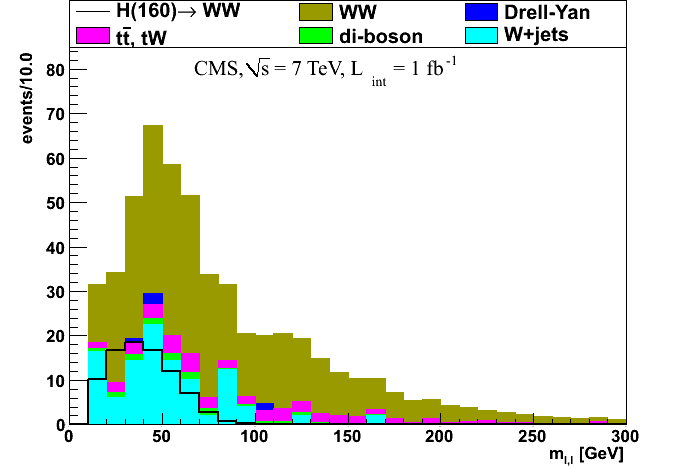
\includegraphics[width=.32\textwidth]{figures/dilepmass_hm160_jets0.png}}
\subfigure[]{
\centering
\label{subfig:dilepmass_hm250_jets0}
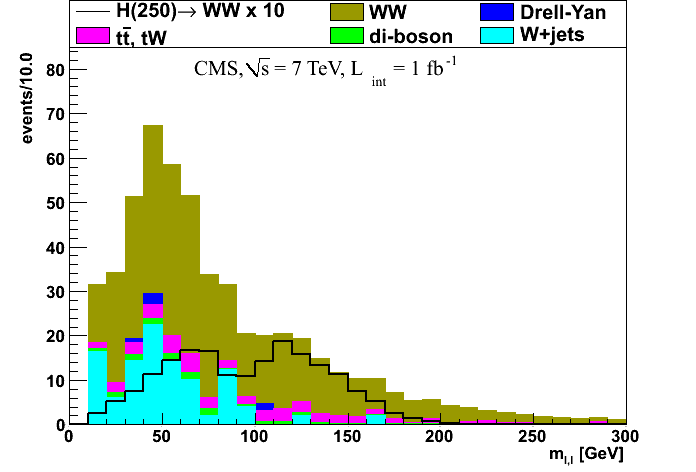
\includegraphics[width=.32\textwidth]{figures/dilepmass_hm250_jets0.png}}\\
\caption{Di-lepton mass distribution after \WW\ selection for $m_H$=120 $\GeVcc$ \subref{subfig:dilepmass_hm120_jets0}, 
$m_H$=160 $\GeVcc$ \subref{subfig:dilepmass_hm160_jets0} and $m_H$=250 $\GeVcc$ \subref{subfig:dilepmass_hm250_jets0} in the 0-jet bin.}
\label{fig:dilepmass_jets0}
\end{figure}

\begin{figure}[!hbtp]
\centering
\subfigure[]{
\centering
\label{subfig:dileppt_hm120_jets0}
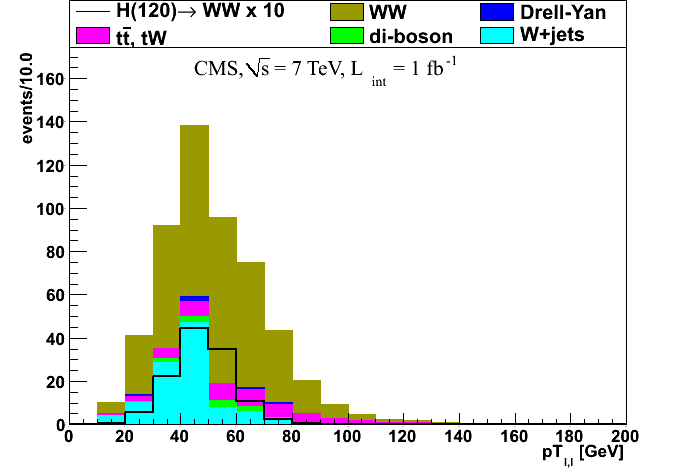
\includegraphics[width=.32\textwidth]{figures/dileppt_hm120_jets0.png}}
\subfigure[]{
\centering
\label{subfig:dileppt_hm160_jets0}
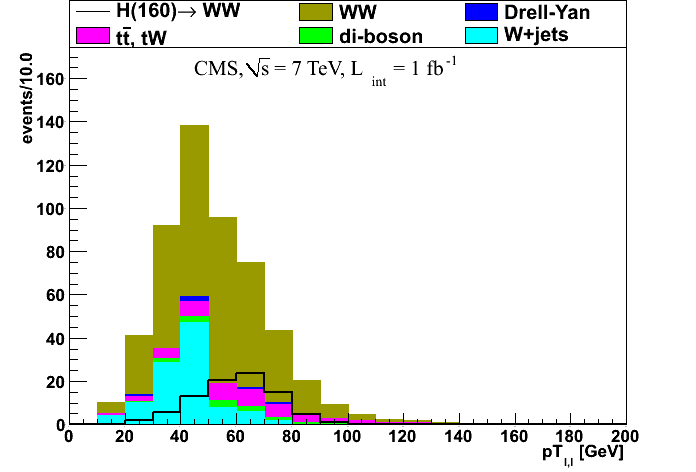
\includegraphics[width=.32\textwidth]{figures/dileppt_hm160_jets0.png}}
\subfigure[]{
\centering
\label{subfig:dileppt_hm250_jets0}
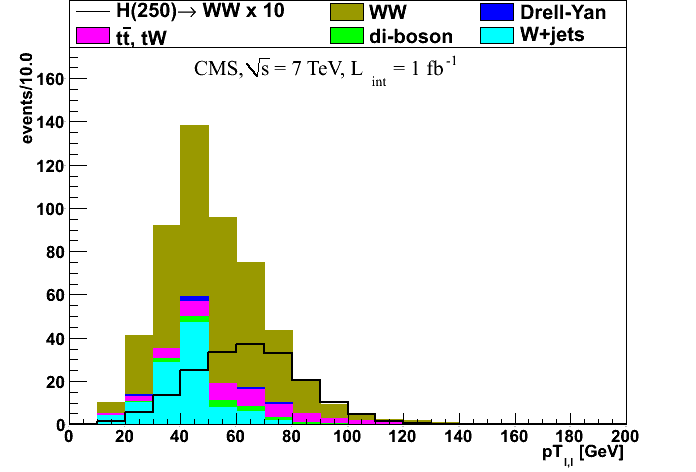
\includegraphics[width=.32\textwidth]{figures/dileppt_hm250_jets0.png}}\\
\caption{Di-lepton $p_T$ distribution after \WW\ selection for $m_H$=120 $\GeVcc$ \subref{subfig:dileppt_hm120_jets0}, 
$m_H$=160 $\GeVcc$ \subref{subfig:dileppt_hm160_jets0} and $m_H$=250 $\GeVcc$ \subref{subfig:dileppt_hm250_jets0} in the 0-jet bin.}
\label{fig:dileppt_jets0}
\end{figure}

\begin{figure}[!hbtp]
\centering
\subfigure[]{
\centering
\label{subfig:mt_hm120_jets0}
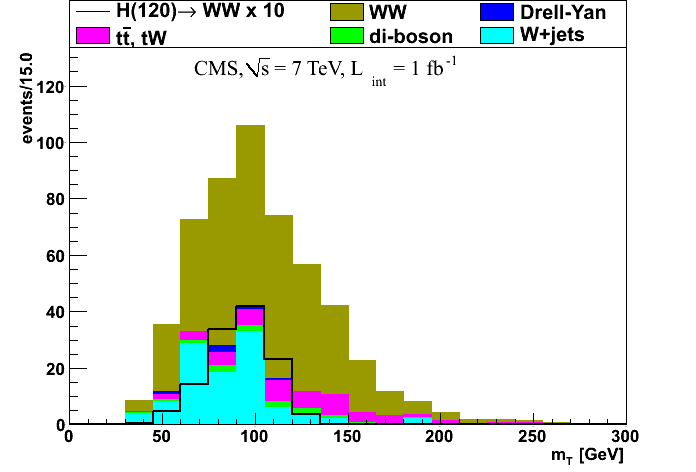
\includegraphics[width=.32\textwidth]{figures/mt_hm120_jets0.png}}
\subfigure[]{
\centering
\label{subfig:mt_hm160_jets0}
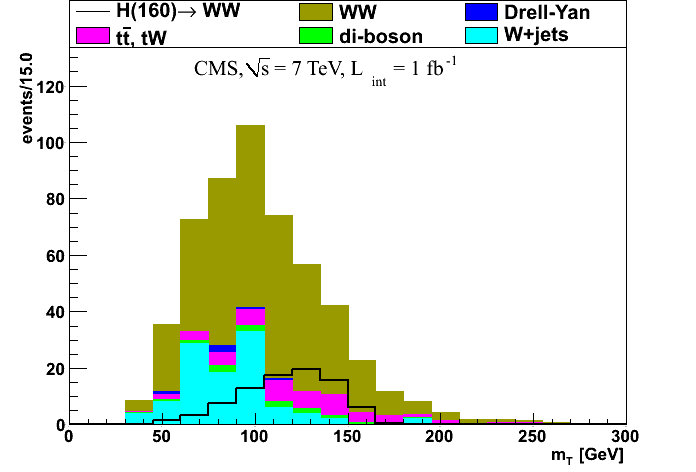
\includegraphics[width=.32\textwidth]{figures/mt_hm160_jets0.png}}
\subfigure[]{
\centering
\label{subfig:mt_hm250_jets0}
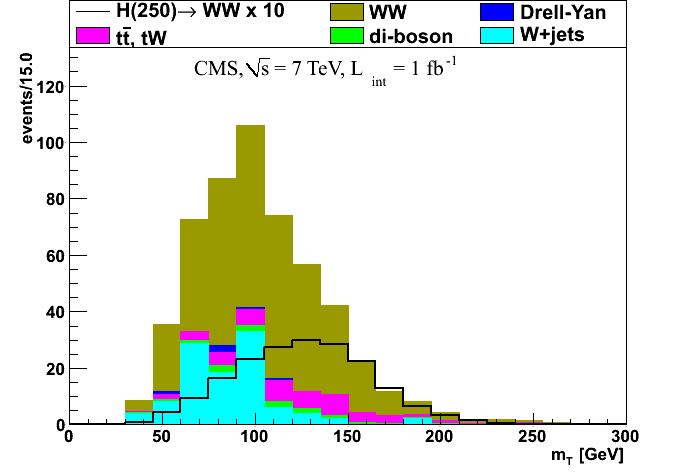
\includegraphics[width=.32\textwidth]{figures/mt_hm250_jets0.png}}\\
\caption{$M_T$ distribution after \WW\ selection for $m_H$=120 $\GeVcc$ \subref{subfig:mt_hm120_jets0}, 
$m_H$=160 $\GeVcc$ \subref{subfig:mt_hm160_jets0} and $m_H$=250 $\GeVcc$ \subref{subfig:mt_hm250_jets0} in the 0-jet bin.}
\label{fig:mt_jets0}
\end{figure}

\begin{figure}[!hbtp]
\centering
\subfigure[]{
\centering
\label{subfig:pmet_hm120_jets0}
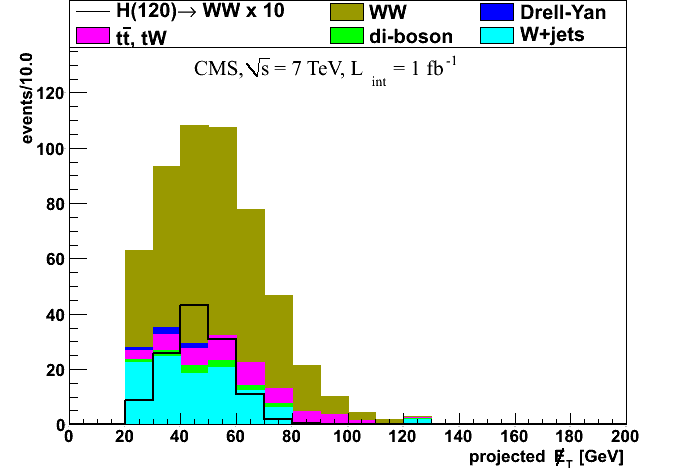
\includegraphics[width=.32\textwidth]{figures/pmet_hm120_jets0.png}}
\subfigure[]{
\centering
\label{subfig:pmet_hm160_jets0}
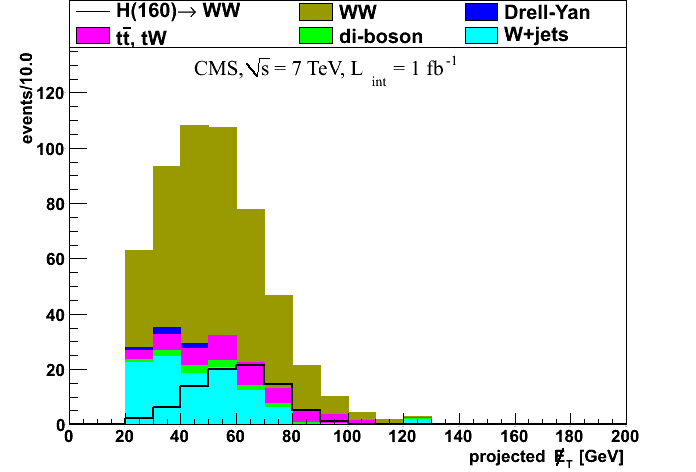
\includegraphics[width=.32\textwidth]{figures/pmet_hm160_jets0.png}}
\subfigure[]{
\centering
\label{subfig:pmet_hm250_jets0}
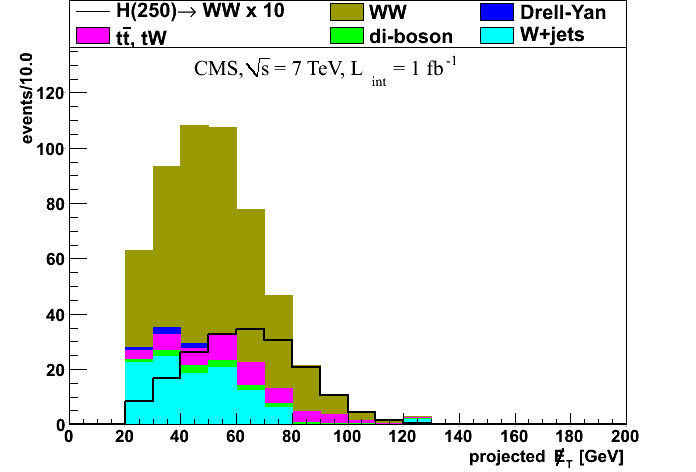
\includegraphics[width=.32\textwidth]{figures/pmet_hm250_jets0.png}}\\
\caption{Projected $\met$ distribution after \WW\ selection for $m_H$=120 $\GeVcc$ \subref{subfig:pmet_hm120_jets0}, 
$m_H$=160 $\GeVcc$ \subref{subfig:pmet_hm160_jets0} and $m_H$=250 $\GeVcc$ \subref{subfig:pmet_hm250_jets0} in the 0-jet bin.}
\label{fig:pmet_jets0}
\end{figure}








\begin{figure}[!hbtp]
\centering
\subfigure[]{
\centering
\label{subfig:dPhi_hm120_jets1}
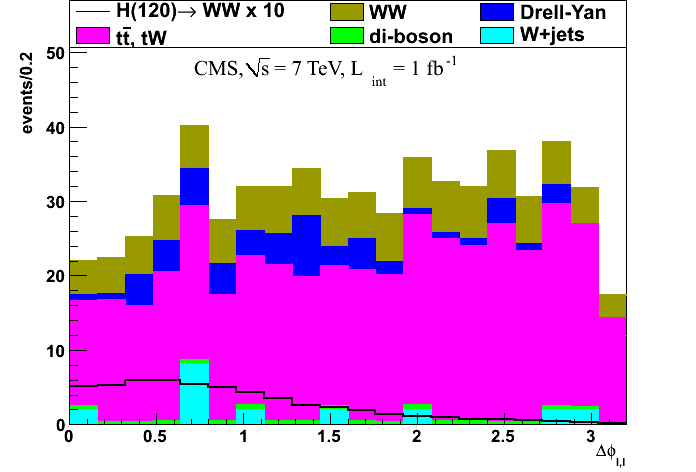
\includegraphics[width=.32\textwidth]{figures/dPhi_hm120_jets1.png}}
\subfigure[]{
\centering
\label{subfig:dPhi_hm160_jets1}
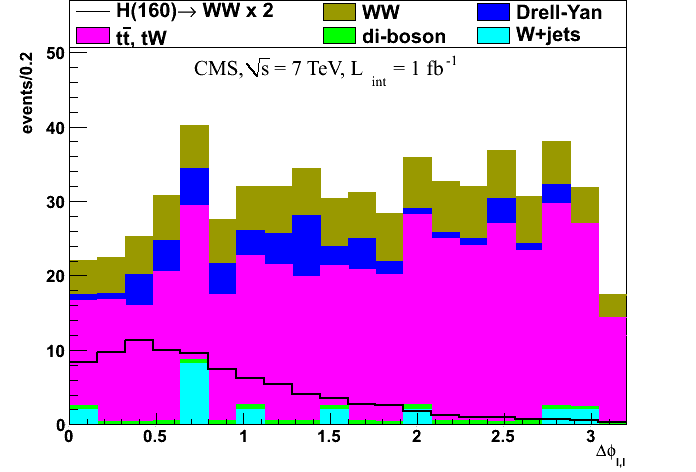
\includegraphics[width=.32\textwidth]{figures/dPhi_hm160_jets1.png}}
\subfigure[]{
\centering
\label{subfig:dPhi_hm250_jets1}
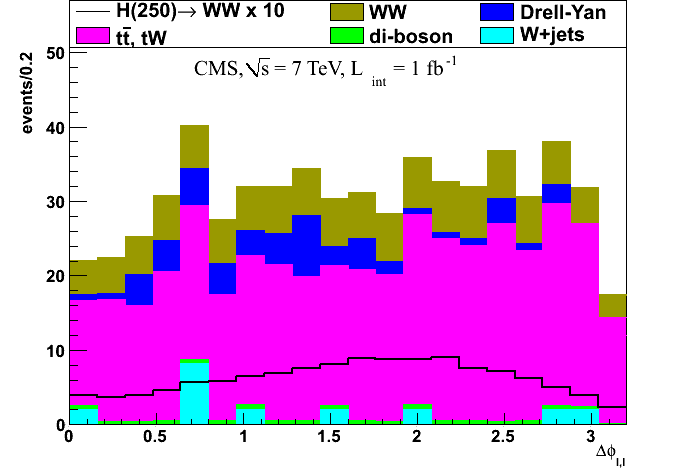
\includegraphics[width=.32\textwidth]{figures/dPhi_hm250_jets1.png}}\\
\caption{Lepton $\Delta\phi$ distribution after \WW\ selection for $m_H$=120 $\GeVcc$ \subref{subfig:dPhi_hm120_jets1}, 
$m_H$=160 $\GeVcc$ \subref{subfig:dPhi_hm160_jets1} and $m_H$=250 $\GeVcc$ \subref{subfig:dPhi_hm250_jets1} in the 1-jet bin.}
\label{fig:dPhi_jets1}
\end{figure}

\begin{figure}[!hbtp]
\centering
\subfigure[]{
\centering
\label{subfig:dilepmass_hm120_jets1}
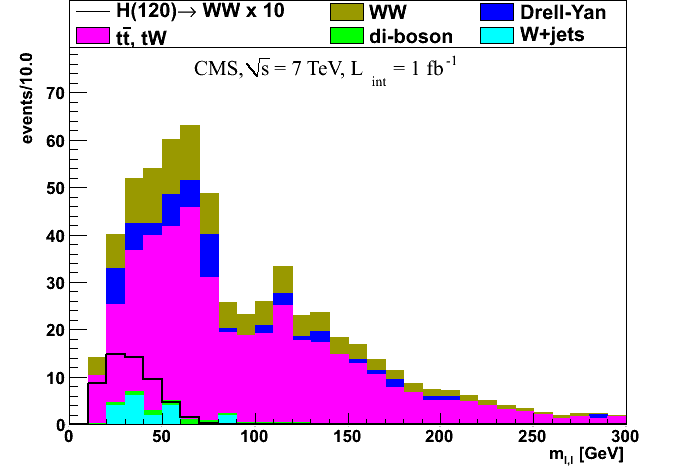
\includegraphics[width=.32\textwidth]{figures/dilepmass_hm120_jets1.png}}
\subfigure[]{
\centering
\label{subfig:dilepmass_hm160_jets1}
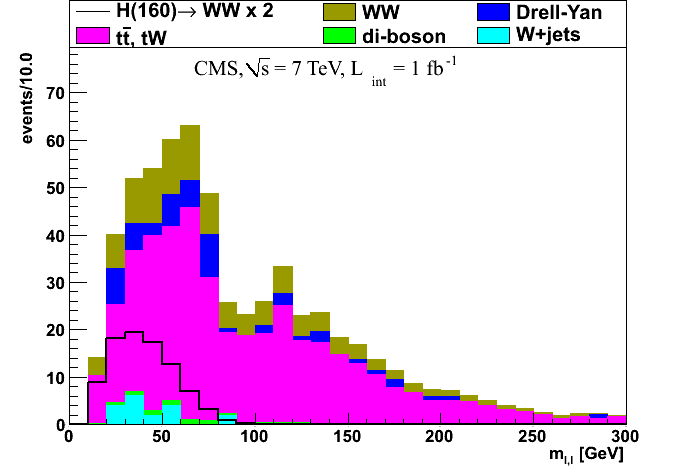
\includegraphics[width=.32\textwidth]{figures/dilepmass_hm160_jets1.png}}
\subfigure[]{
\centering
\label{subfig:dilepmass_hm250_jets1}
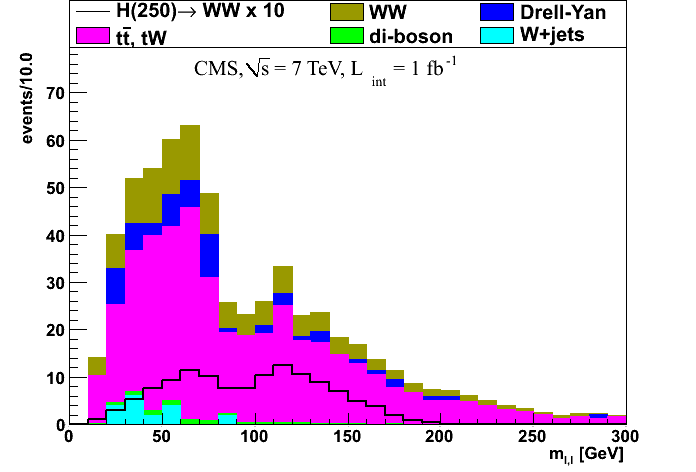
\includegraphics[width=.32\textwidth]{figures/dilepmass_hm250_jets1.png}}\\
\caption{Di-lepton mass distribution after \WW\ selection for $m_H$=120 $\GeVcc$ \subref{subfig:dilepmass_hm120_jets1}, 
$m_H$=160 $\GeVcc$ \subref{subfig:dilepmass_hm160_jets1} and $m_H$=250 $\GeVcc$ \subref{subfig:dilepmass_hm250_jets1} in the 1-jet bin.}
\label{fig:dilepmass_jets1}
\end{figure}

\begin{figure}[!hbtp]
\centering
\subfigure[]{
\centering
\label{subfig:dileppt_hm120_jets1}
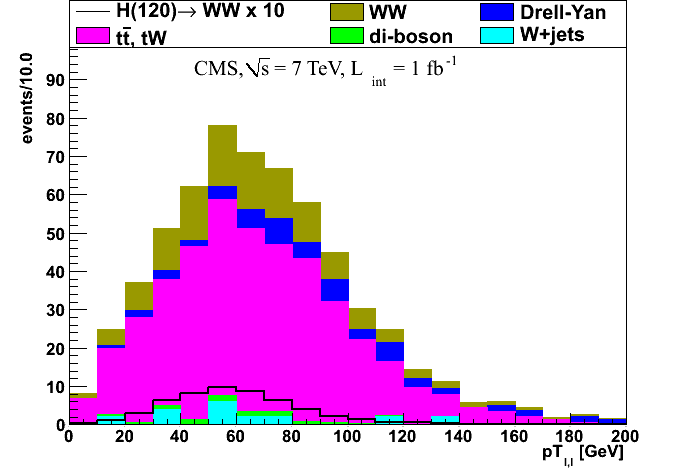
\includegraphics[width=.32\textwidth]{figures/dileppt_hm120_jets1.png}}
\subfigure[]{
\centering
\label{subfig:dileppt_hm160_jets1}
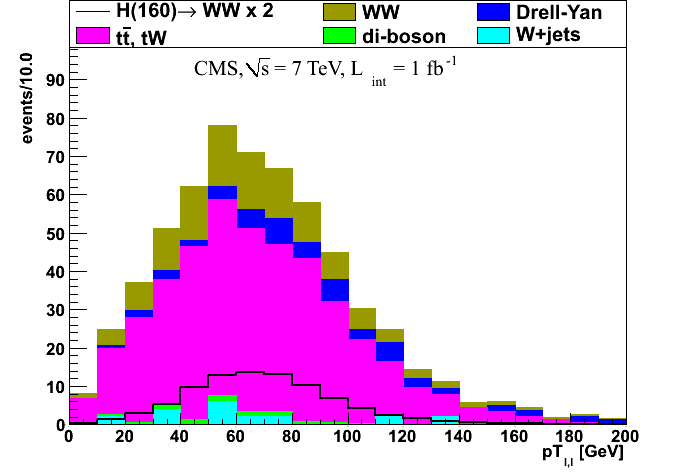
\includegraphics[width=.32\textwidth]{figures/dileppt_hm160_jets1.png}}
\subfigure[]{
\centering
\label{subfig:dileppt_hm250_jets1}
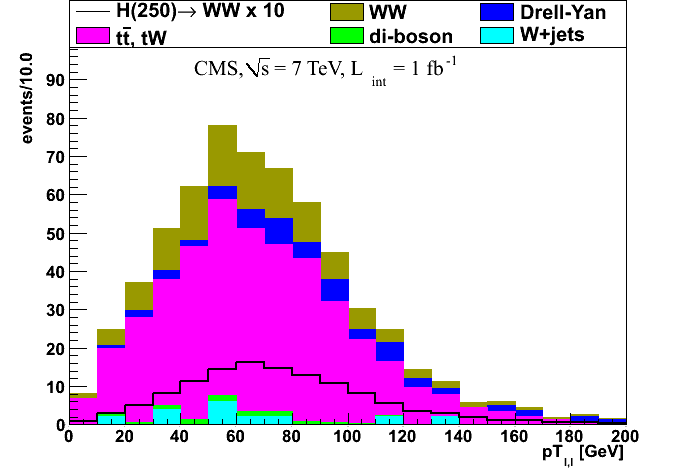
\includegraphics[width=.32\textwidth]{figures/dileppt_hm250_jets1.png}}\\
\caption{Di-lepton $p_T$ distribution after \WW\ selection for $m_H$=120 $\GeVcc$ \subref{subfig:dileppt_hm120_jets1}, 
$m_H$=160 $\GeVcc$ \subref{subfig:dileppt_hm160_jets1} and $m_H$=250 $\GeVcc$ \subref{subfig:dileppt_hm250_jets1} in the 1-jet bin.}
\label{fig:dileppt_jets1}
\end{figure}

\begin{figure}[!hbtp]
\centering
\subfigure[]{
\centering
\label{subfig:mt_hm120_jets1}
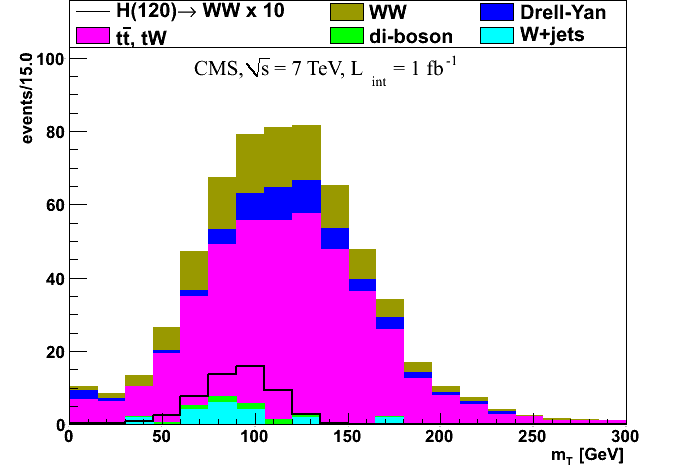
\includegraphics[width=.32\textwidth]{figures/mt_hm120_jets1.png}}
\subfigure[]{
\centering
\label{subfig:mt_hm160_jets1}
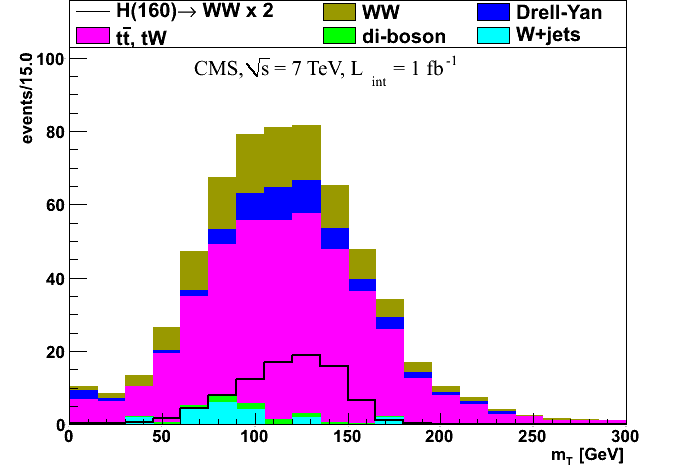
\includegraphics[width=.32\textwidth]{figures/mt_hm160_jets1.png}}
\subfigure[]{
\centering
\label{subfig:mt_hm250_jets1}
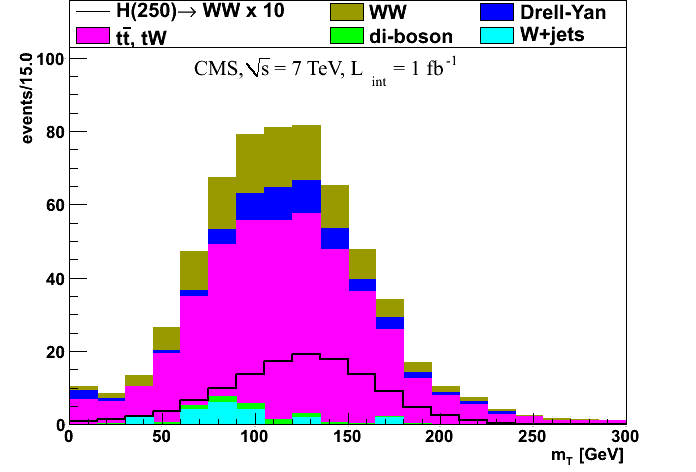
\includegraphics[width=.32\textwidth]{figures/mt_hm250_jets1.png}}\\
\caption{$M_T$ distribution after \WW\ selection for $m_H$=120 $\GeVcc$ \subref{subfig:mt_hm120_jets1}, 
$m_H$=160 $\GeVcc$ \subref{subfig:mt_hm160_jets1} and $m_H$=250 $\GeVcc$ \subref{subfig:mt_hm250_jets1} in the 1-jet bin.}
\label{fig:mt_jets1}
\end{figure}

\begin{figure}[!hbtp]
\centering
\subfigure[]{
\centering
\label{subfig:pmet_hm120_jets1}
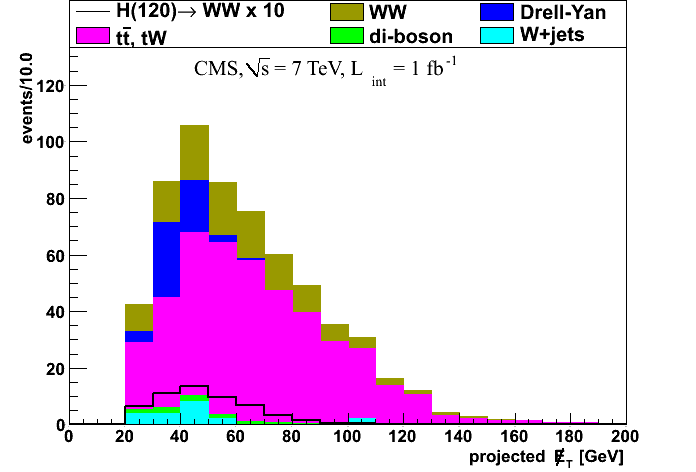
\includegraphics[width=.32\textwidth]{figures/pmet_hm120_jets1.png}}
\subfigure[]{
\centering
\label{subfig:pmet_hm160_jets1}
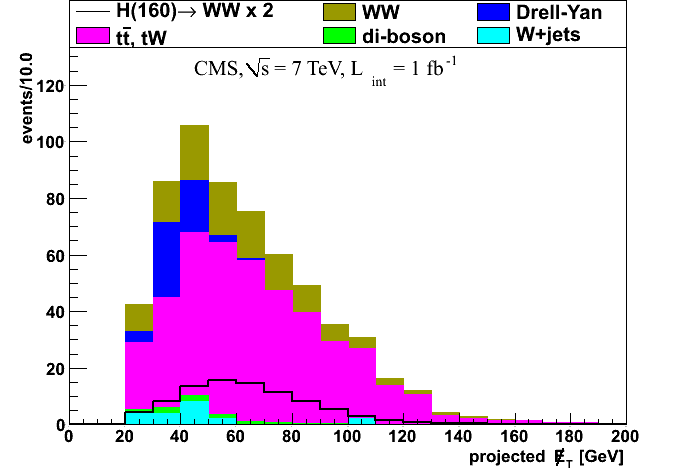
\includegraphics[width=.32\textwidth]{figures/pmet_hm160_jets1.png}}
\subfigure[]{
\centering
\label{subfig:pmet_hm250_jets1}
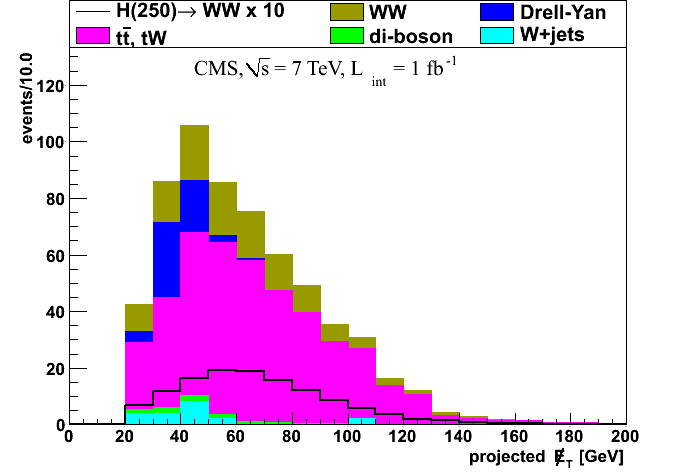
\includegraphics[width=.32\textwidth]{figures/pmet_hm250_jets1.png}}\\
\caption{Projected $\met$ distribution after \WW\ selection for $m_H$=120 $\GeVcc$ \subref{subfig:pmet_hm120_jets1}, 
$m_H$=160 $\GeVcc$ \subref{subfig:pmet_hm160_jets1} and $m_H$=250 $\GeVcc$ \subref{subfig:pmet_hm250_jets1} in the 1-jet bin.}
\label{fig:pmet_jets1}
\end{figure}
